%% LyX 2.3.6 created this file.  For more info, see http://www.lyx.org/.
%% Do not edit unless you really know what you are doing.
\documentclass[10pt]{article}
\usepackage{helvet}
\renewcommand{\familydefault}{\sfdefault}
\usepackage[T1]{fontenc}
\usepackage[latin9]{inputenc}
\usepackage[a4paper]{geometry}
\geometry{verbose,tmargin=2cm,bmargin=4cm,lmargin=2cm,rmargin=2cm}
\usepackage{fancyhdr}
\pagestyle{fancy}
\setlength{\parskip}{6pt}
\setlength{\parindent}{0pt}
\usepackage{tcolorbox}
\usepackage{amsmath}
\usepackage{amsthm}
\usepackage{amssymb}
\usepackage{graphicx}

\makeatletter

%%%%%%%%%%%%%%%%%%%%%%%%%%%%%% LyX specific LaTeX commands.
%% A simple dot to overcome graphicx limitations
\newcommand{\lyxdot}{.}


%%%%%%%%%%%%%%%%%%%%%%%%%%%%%% User specified LaTeX commands.
\usepackage{tcolorbox}
\usepackage{amsthm}
\usepackage{lastpage}
\usepackage{fancyhdr}
\usepackage{accents}
\usepackage{titlesec}
\usepackage{marginnote}


\usepackage{enumitem}
\setlist{nolistsep}

\usepackage{tcolorbox}
\definecolor{light-blue}{cmyk}{0.24, 0.12, 0.0, 0.04, 1.00}


%

%parskip shold take care of heading spacing
\titlespacing\section{0pt}{0pt}{0pt}
\titlespacing\subsection{0pt}{0pt}{0pt}
\titlespacing\subsubsection{0pt}{0pt}{0pt}



\setlength{\headheight}{40pt}

\makeatother

\begin{document}
\lhead{Group 17} \rhead{CS7NS1 Project 3 Report} 

% TODO: declaration?
% \begin{tcolorbox}[colback=light-blue]
% \begin{small} \textbf{DECLARATION:} I understand that this is an
% \textbf{individual} assessment and that collaboration is not permitted.
% I have read, understand and agree to abide by the plagiarism provisions
% in the General Regulations of the University Calendar for the current
% year, found at http://www.tcd.ie/calendar. I understand that by returning
% this declaration with my work, I am agreeing with the above statement.
% \end{small} 
% \end{tcolorbox}

\bigskip{}

\section{Introduction}

\section{Oceanography Scenario Description and Motivation}


Our protocol is peer-to-peer, where peer-to-peer
here means communication between
a pair of nodes with a direct physical link (acoustic, RF, fibre, what have you).

\section{ICN/NDN Protocol}
Here we describe our ICN/NDN protocol which we name G17ICN 1.0.
\subsection{Concise Description of the Protocol}
The protocol uses HTTP as the serialization and request/response format, with a JWT as the request body.
There are two types of ICN packets in our protocol, interest and satisfy packets.
Interest and satisfy packets are encoded as JWTs
and delivered in the body of a HTTP POST request.

The JWTs are signed using PKC, the default algorithm in our emulation is RSA 256 with key size 512, but this is configurable.
Both interest and satisfy packets are signed.

Timestamps in the protocol are seconds since the epoch, either integer or decimal.

Satisfy packets are sent lazily, i.e. only after receiving a corresponding interest packet.

\subsubsection{Optimisation Headers}
Our protocol uses HTTP headers to provide hints to neighbouring nodes for routing optimisation.
The `x-g17icn-version` will facilitate compatibility with future version of the protocol.
The `x-g17icn-hopcount` header indicates the distance in hops that a packet has traveled from its origin.
A series of headers `x-g17icn-router-0`, `x-g17icn-router-1`, etc. allow each router to reconstruct the traceroute of the packet so far.
This can also be used for a router to gleem an approximate picture of the network topology. The `x-g17icn-router-X` headers contain three pieces of information; 1. the time at which the router first received the packet, 2. the key name of the router, 3. a numeric indicator of the router's congestion at that time.

\begin{figure}
	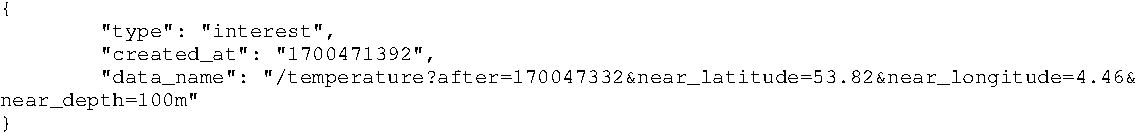
\includegraphics[width=1\textwidth]{example_interest_packet.json.pdf}	
	\caption{\label{fig:interest-packet-json}An example of the JSON data for an interest packet that will be encoded as a JWT.}
\end{figure}


Our protocol uses HTTP 1.1 as the serialization standard, and in the emulation the HTTP request and response messages are delivered over TCP.
HTTP is a request/response style standard; a client makes a request to a server and the server responds.
The responses in our protocol are merely acknowledgment responses intended to inform the client as to whether
the request is being processed. The HTTP response does not contain data to satisfy the request.
Each device in the network runs a HTTP server listening to respond to requests.

\subsection{Motivation and Design Considerations}
\subsection{Security}

All interest and satisfy packets are signed by the creator of the packet
such that any node can verify the authenticity of a message.
PKC is used, so each node has a public-private key pair.
The node uses it's private key to create a cryptographic signature of the
interest/satisfy packet, and encodes the packet and signature as a JWT.

\section{Emulation}
We have implementented an {\em emulation} of our protocol, not a deployable implementation of the protocol,
for the reason that an emulation facilitates more thorough evaluation and debugging.
In the scenario we have described it is assumed that devices would communicate with each other primarily over acoustic links
but we have not emulated characteristics of the physical layer.
Rather, our focus has been on emulating diverse and dynamic network topologies.

In the emulation each device finds for itself a unique IP interface (host/port pair).

\end{document}
